\documentclass[
12pt, % Main document font size
a4paper, % Paper type, use 'letterpaper' for US Letter paper
oneside,
% One page layout (no page indentation)
%twoside, % Two page layout (page indentation for binding and different headers)
%hidelinks, % Hide links like hyperref
%headinclude,footinclude, % Extra spacing for the header and footer
%BCOR5mm, % Binding correction
]{article}



\setlength{\parindent}{5pt} %Modifica la dimensione dell'indentazione dei paragrafi



%%%%% Packages
%\usepackage [english]{babel}
\usepackage [italian]{babel}

\usepackage{enumitem} % migliori enumerate, ad esempio \begin{enumerate}[label=\Alph*]

%per far chiudere e aprire " "
%\usepackage [autostyle, english = american]{csquotes}
%\MakeOuterQuote{"}

\usepackage{hyphenat}
\begin{hyphenrules}{english}
\hyphenation{Fortran}
\hyphenation{spa-sti-ci-ty} 
\end{hyphenrules}

\usepackage[section]{placeins} %Also one can consider the placeins package and the \FloatBarrier command that prevents figures from floating any further. If figures are supposed to remain in the section, one can load

\usepackage{tabularx} %advance tables, like wrap text inside cell
\usepackage{longtable}

\usepackage{graphicx}
%\usepackage{subfig}
\usepackage{xcolor} %Colori Aggiuntiv
\usepackage[colorlinks = true,
	linkcolor = teal,
	urlcolor  = blue,
	citecolor = teal,
	anchorcolor = blue]{hyperref} %Hyperref
	
% listings for code	
\usepackage{listings}
\usepackage{color}
\definecolor{dkgreen}{rgb}{0,0.8,0}
\definecolor{gray}{rgb}{0.5,0.5,0.5}
\definecolor{mauve}{rgb}{0.58,0,0.82}

\lstset{frame=shadowbox,
  language=Matlab,
  aboveskip=3mm,
  belowskip=3mm,
  showstringspaces=false,
  columns=flexible,
  basicstyle={\small\ttfamily},
  numbers=none,
  numberstyle=\tiny\color{gray},
  keywordstyle=\color{blue},
  commentstyle=\color{dkgreen},
  stringstyle=\color{mauve},
  breaklines=true,
  breakatwhitespace=true,
  tabsize=3
}


\usepackage{url}

%\usepackage{lipsum} %Crea dummy text

\usepackage{amsmath,amssymb,amscd,amsfonts,amsthm} %Roba matematica

%bibliografia
%\usepackage[shortalphabetic,abbrev]{amsrefs}
%\usepackage[author-year, y2k]{amsrefs}
\usepackage[alphabetic]{amsrefs}
\usepackage{mathtools}

\usepackage{physics}

\usepackage{siunitx} %database unita` di misura, \si{ \kg \per \second},  \SI{20}{ \kg \per \second}
\sisetup{
	round-mode          = places,
	round-precision     = 2,
}

\usepackage{gensymb} %simboli extra, come \degree

\usepackage{tikz}
	\usetikzlibrary{shapes,arrows}
	\tikzstyle{block} = [draw, fill=white, rectangle, 
	minimum height=3em, minimum width=6em]
	\tikzstyle{sum} = [draw, fill=white, circle, node distance=1cm]
	\tikzstyle{input} = [coordinate]
	\tikzstyle{output} = [coordinate]
	\tikzstyle{pinstyle} = [pin edge={to-,thin,black}]
	\usepackage{tikzscale}

\usepackage{pgfplots}
	\pgfplotsset{width=7cm,compat=1.14}
	%\pgfplotsset{compat=newest} % Allows to place the legend below plot
	\pgfplotsset{every minor tick/.append style={thin}}  % applies only to minor ticks,
	\usepgfplotslibrary{units} % Allows to enter the units nicely
	%\usepgfplotslibrary{external} 
	%\tikzexternalize
	%\tikzset{external/force remake}
	\pgfkeys{/pgf/number format/.cd,1000 sep={\,}}

\usepackage{afterpage}

\usepackage{comment} % inserisce la funzionalita` \begin{comment}
\usepackage{wrapfig}
\usepackage{vmargin}
\setmarginsrb  {25mm}  % left margin
	{ 5mm}  % top margin
	{25mm}  % right margin
	{15mm}  % bottom margin
	{10mm}  % head height
	{15mm}  % head sep
	{10mm}  % foot height
	{15mm}  % foot sep

% permettono l'uso di subfigures
\usepackage{caption}
\usepackage{subcaption}


%%%%%%%%%%%%%%%%%%%%%%%%%%%%%%%%%%%%%%%%%%%%%%%%%%%%%%%%%%
%%%%% Comandi homebrewed


%% comando per fare matrix con linee verticali. Esempio:
%\[
%\begin{pmatrix}[cc|c]
%  1 & 2 & 3\\
%  4 & 5 & 9
%\end{pmatrix}
%\]
\makeatletter
\renewcommand*\env@matrix[1][*\c@MaxMatrixCols c]{%
  \hskip -\arraycolsep
  \let\@ifnextchar\new@ifnextchar
  \array{#1}}
\makeatother


%% renew comando paragraph per far andare a capo dopo \paragraph
\newcommand{\myparagraph}[1]{\paragraph{#1}\mbox{}\\}

\newcommand{\bs}{\textbackslash}

%% BLANKPAGE
%per creare pagine vuote
\newcommand\blankpage{%
	\null
	\thispagestyle{empty}%
	%\addtocounter{page}{-1}%
	\newpage}

%% RNUM 
% porta in numeri romani il unmero
\newcommand{\RNum}[1]{\uppercase\expandafter{\romannumeral #1\relax}}

%% AT
% Comando per le derivate calcolate nel punto. Esempio: \dv{\text{Im}T(j \omega)}{t} \at[\Big]{\omega = \omega_1}
\newcommand{\at}[2][]{#1|_{#2}}

%% Comando per valori assoluti che scalano
%\DeclarePairedDelimiter\abs{\lvert}{\rvert}%
%\DeclarePairedDelimiter\norm{\lVert}{\rVert}%
% Swap the definition of \abs* and \norm*, so that \abs
% and \norm resizes the size of the brackets, and the 
% starred version does not.
\makeatletter
\let\oldabs\abs
\def\abs{\@ifstar{\oldabs}{\oldabs*}}
%
%\let\oldnorm\norm
%\def\norm{\@ifstar{\oldnorm}{\oldnorm*}}
\makeatother

%% CEILING and FLOOR
\DeclarePairedDelimiter\ceil{\lceil}{\rceil}
\DeclarePairedDelimiter\floor{\lfloor}{\rfloor}

% %% Prova theorem
% \newtheorem{theorem}{Theorem}[section]
% \newtheorem{lemma}[theorem]{Lemma}
% \newtheorem{proposition}[theorem]{Proposition}
% \newtheorem{corollary}[theorem]{Corollary}

% \newenvironment{Proof}[1][Proof]{\begin{trivlist}
% 		\item[\hskip \labelsep {\bfseries #1}]}{\end{trivlist}}
% \newenvironment{definition}[1][Definition]{\begin{trivlist}
% 		\item[\hskip \labelsep {\bfseries #1}]}{\end{trivlist}}
% \newenvironment{example}[1][Example]{\begin{trivlist}
% 		\item[\hskip \labelsep {\bfseries #1}]}{\end{trivlist}}
% \newenvironment{remark}[1][Remark]{\begin{trivlist}
% 		\item[\hskip \labelsep {\bfseries #1}]}{\end{trivlist}}

%\newcommand{\qed}{\nobreak \ifvmode \relax \else
%	\ifdim\lastskip<1.5em \hskip-\lastskip
%	\hskip1.5em plus0em minus0.5em \fi \nobreak
%	\vrule height0.75em width0.5em depth0.25em\fi}

%% \xoverline
% simile a \bar ma copre tutta il width della lettera
\makeatletter
\newsavebox\myboxA
\newsavebox\myboxB
\newlength\mylenA

\newcommand*\xoverline[2][0.75]{%
    \sbox{\myboxA}{$\m@th#2$}%
    \setbox\myboxB\null% Phantom box
    \ht\myboxB=\ht\myboxA%
    \dp\myboxB=\dp\myboxA%
    \wd\myboxB=#1\wd\myboxA% Scale phantom
    \sbox\myboxB{$\m@th\overline{\copy\myboxB}$}%  Overlined phantom
    \setlength\mylenA{\the\wd\myboxA}%   calc width diff
    \addtolength\mylenA{-\the\wd\myboxB}%
    \ifdim\wd\myboxB<\wd\myboxA%
       \rlap{\hskip 0.5\mylenA\usebox\myboxB}{\usebox\myboxA}%
    \else
        \hskip -0.5\mylenA\rlap{\usebox\myboxA}{\hskip 0.5\mylenA\usebox\myboxB}%
    \fi}
\makeatother

%%



\graphicspath{{./figs/}}

\begin{document}
	
\begin{titlepage}
	\centering
	\vspace*{0.0 cm}
	
\includegraphics[height=.2\textheight]{figs/cherubino_pant541.pdf}\\[0.5 cm]			% University Logo
	\textsc{\Large Universit\`a di Pisa }\\[0.5 cm]							% University Name
	\textsc{\large Laurea Magistrale \\ 
		\vspace{2mm} in Ingegneria Robotica e dell'Automazione}\\[0.5 cm]
	\textsc{Progetto di Sistemi di Guida e Navigazione}\\[0.25 cm]	
	
	\rule{\linewidth}{0.2 mm} \\[0.4 cm]
	{ \Large{\textbf{Navigazione attraverso AMCL e sistema UWB}}}\\
	\rule{\linewidth}{0.2 mm} \\[0.5 cm]
	%\vspace*{0.5 cm}
	
	\includegraphics[height=0.3\textheight]{charlie_vista_assonometrica.pdf}\\	
	\vspace{1 cm}
	
	
	\begin{minipage}{0.48\textwidth}
		\begin{flushleft}
			\textit{Autori:}\\
			Alessia Biondi\\
			Francesco Petracci
			
			
		\end{flushleft}
	\end{minipage}~
	\begin{minipage}{0.48\textwidth}
		\begin{flushright}    
			\textit{Professore:}\\		
			Lorenzo Pollini\\
		\end{flushright}
	\end{minipage}\\[2 cm]

	
\end{titlepage}
\newpage

% pagina vuota e indice
\newpage\null\thispagestyle{empty}\newpage
\newpage
\pagenumbering{arabic}
\setcounter{page}{1}
\tableofcontents
\newpage

%%%%%%%%%%%%%%%%%%%%%%%%%%%%%% 
% TO DO
%	1.
%	2.
%	3.
%
%
%%%%%%


%%%%%%%%%%%%%%%%%%%%%%%%%%%%%%%%%%%%%%%%%%%%%%%%%%%%%%%%%%%%%%%%%%%%%%%%%%%%%%%%%%%%%%%%%%%%%%%%%%%%%%
% introduzione
\section*{Introduzione}
L'obiettivo di questo progetto \`e stato quello di migliorare lo stato del veicolo, partendo dal risolvere le molte problematiche accumulatesi nel passaggio di testimone tra i gruppi precedenti.
Lo scopo principale dell'intero sistema, composto dal veicolo affiancato da una serie di sensori, \`e quello di riuscire a localizzarsi all'interno di una mappa preacquisita e di navigare al suo interno.
La posizione \`e ottenuta seguendo due metodologie tra loro complementari: da una parte viene sfruttato un lidar montato sul corpo del veicolo, che permette di avere buoni risultati in ambienti chiusi in cui siano presenti pareti e confini ben precisi, dall'altra si appoggia ad un sistema Ultra Wide Band (UWB), che ha invece performance migliori in ambienti esterni e privi di ostacoli, sui quali il segnale potrebbe avere interferenze dovute a scattering.
\`E importante sottolineare fin da subito che, tramite il lidar, non viene effettuata una SLAM vera e propria bens\`i uno Scan Matching: infatti, l'algoritmo di localizzazione in condizioni nominali prende come posa del veicolo quella ottenuta dallo scan matcher. 
Quest'ultima viene quindi periodicamente confrontata con quella misurata dal sistema UWB, la quale non rappresenta, in condizioni standard, un indice della posizione del veicolo. Solo nel momento in cui i due valori, restituiti da Lidar e UWB, differiscono di molto, allora l'ultima posa ottenuta dalle antenne viene assegnata al veicolo stesso come sua posa attuale.
In questo modo si ottiene un sistema robusto alla perdita del lidar, che pu\`o verificarsi a seguito di una rottura del sensore o nel momento in cui sono esplorati ambienti dove le condizioni non permettono di avere misure affidabili.

\subsection*{Funzionamento in due parole}
Molto sinteticamente andiamo a descrivere il funzionamento di Charlie. 
In primis viene utilizzato il pacchetto hector-slam allo scopo di pre-acquisire e realizzare una mappa dell'ambiente nel quale il veicolo dovrà poi muoversi. 
Solo in un secondo momento, utilizzando questa mappa, avrà luogo la fase di moto, durante la quale il sistema riesce a localizzarsi nell'ambiente attraverso l'algoritmo Adaptive Monte Carlo Localization, nel quale ha luogo il confronto tra le misure acquisite dal lidar e le feature della mappa stessa. 

Dato che questo algoritmo pu\`o convergere su una posa del veicolo non corretta a causa, per esempio, di ambiguit\`a  tra simmetrie della mappa 
il sistema UWB fa s\`i che venga reinizializzato l'algoritmo AMCL. 
In questo utilizzo quindi il sistema UWB serve solamente come check.

\subsection*{Come ottenere codice}
Il codice sviluppato \`e disponibile nella repository \href{https://github.com/ABiondi12/project_sgn}{github} e un backup del catkin workspace sul 
\href{https://drive.google.com/drive/folders/1rXppVs0qSfeEKQumRFrPhkpiYDCvTXOL?usp=sharing}{Google Drive} associato a Charlie. 
e mini organizzazione \textbf{FARE ALLA FINE QUANDO PRESENTIAMO IL CODICE}


%%%%%%%%%%%%%%%%%%%%%%%%%%%%%%%%%%%%%%%%%%%%%%%%%%%%%%%%%%%%%%%%%%%%%%%%%%%%%%%%%%%%%%%%%%%%%%%%%%%%%%
% descrizione hardware
\newpage
\section{Descrizione Hardware}

Il veicolo, per gli amici e i lettori Charlie, \`e basato su un Crawler RC, una piattaforma meccanica radio--comandata,  su cui sono stati installati dei sensori e delle schede elettroniche. 

A bordo si trovano quindi due unit\`a centrali:
\begin{itemize}
	\item un Raspberry Pi 4 (8Gb Ram), con sistema operativo Linux 18.04 su cui viene eseguito Robot Operating System (ROS)
	\item una scheda STM32F407 connessa ad una pcb Icaro su cui è implementato il sistema di guida e alcuni filtraggi
\end{itemize}

Come sensori sono presenti:
\begin{itemize}
	\item Lidar Slamtec RPLIDAR-A3
	
	\item due tag del sistema UWB creato da Pozyx che dialogano con 4 anchors disposte nell'ambiente
\end{itemize}

\subsubsection*{Alimentazione e Connessioni}

\begin{figure}[] 
	\centering    
	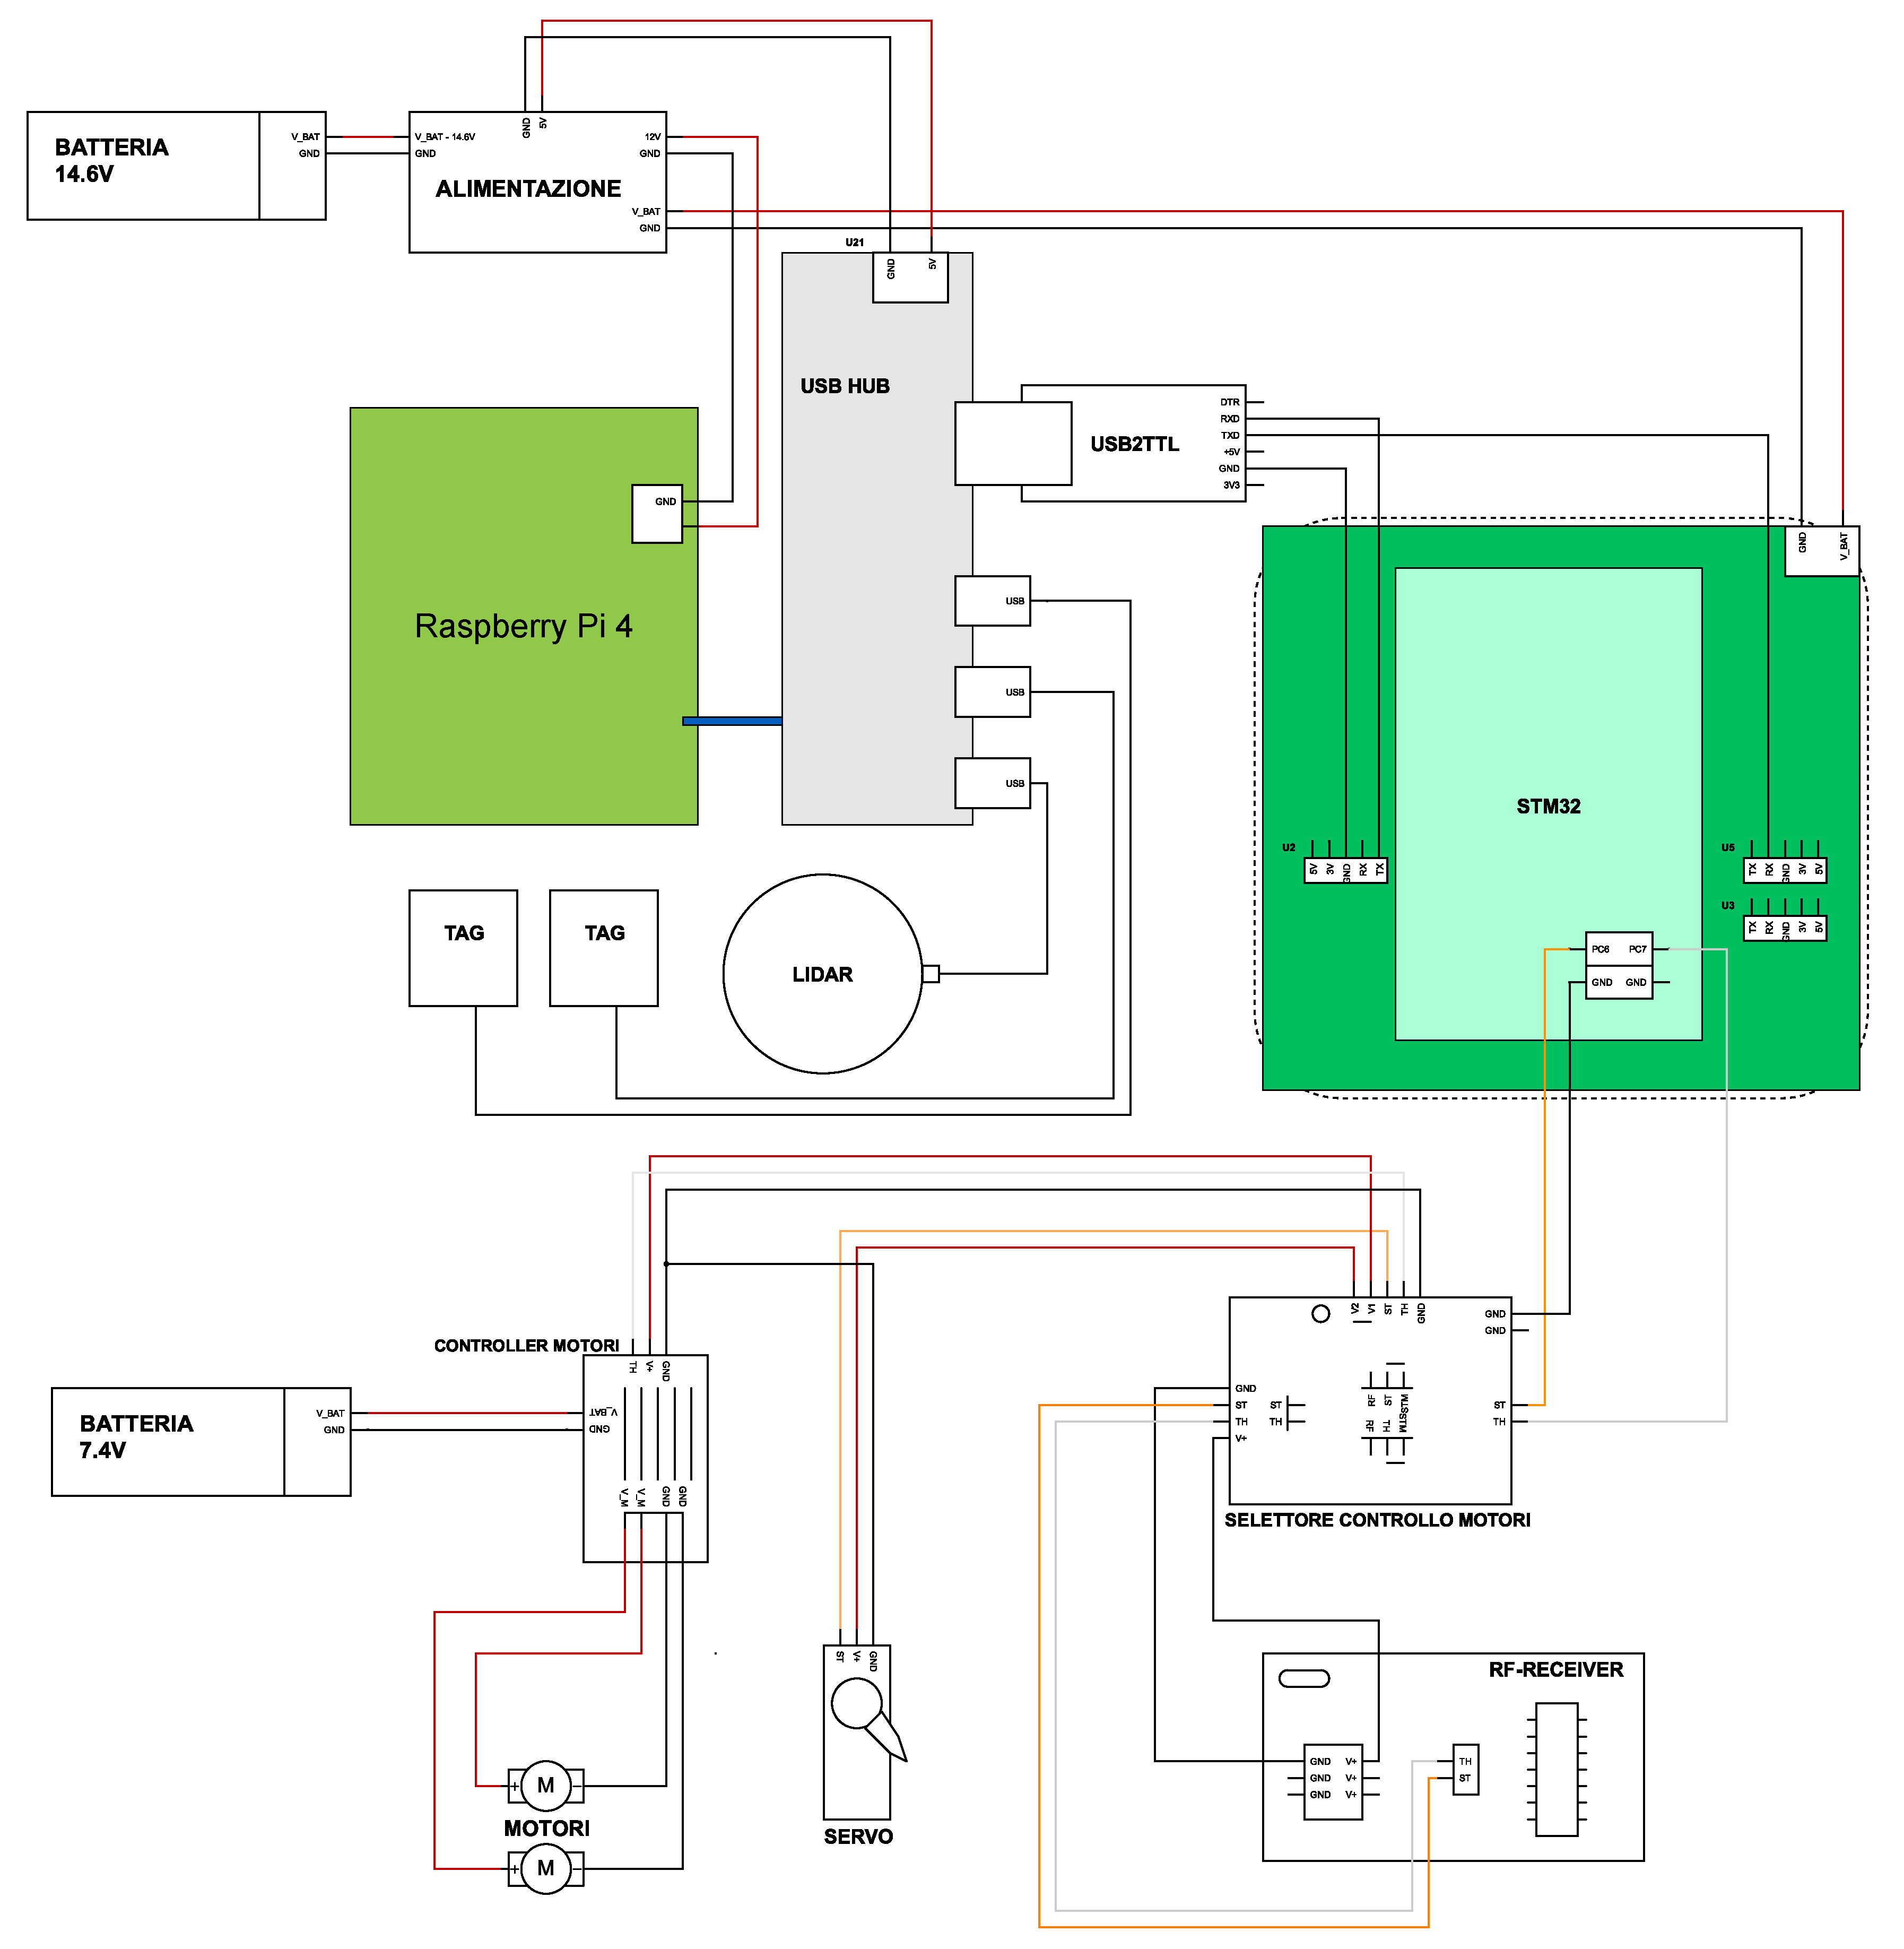
\includegraphics[width=1\textwidth]{schema_completo.pdf}
	\caption{Schema connessioni completo. \textbf{DA EDITARE CON RASPBERRY}}
	\label{fig:schema_completo}
\end{figure}

\begin{figure}[] 
	\centering
	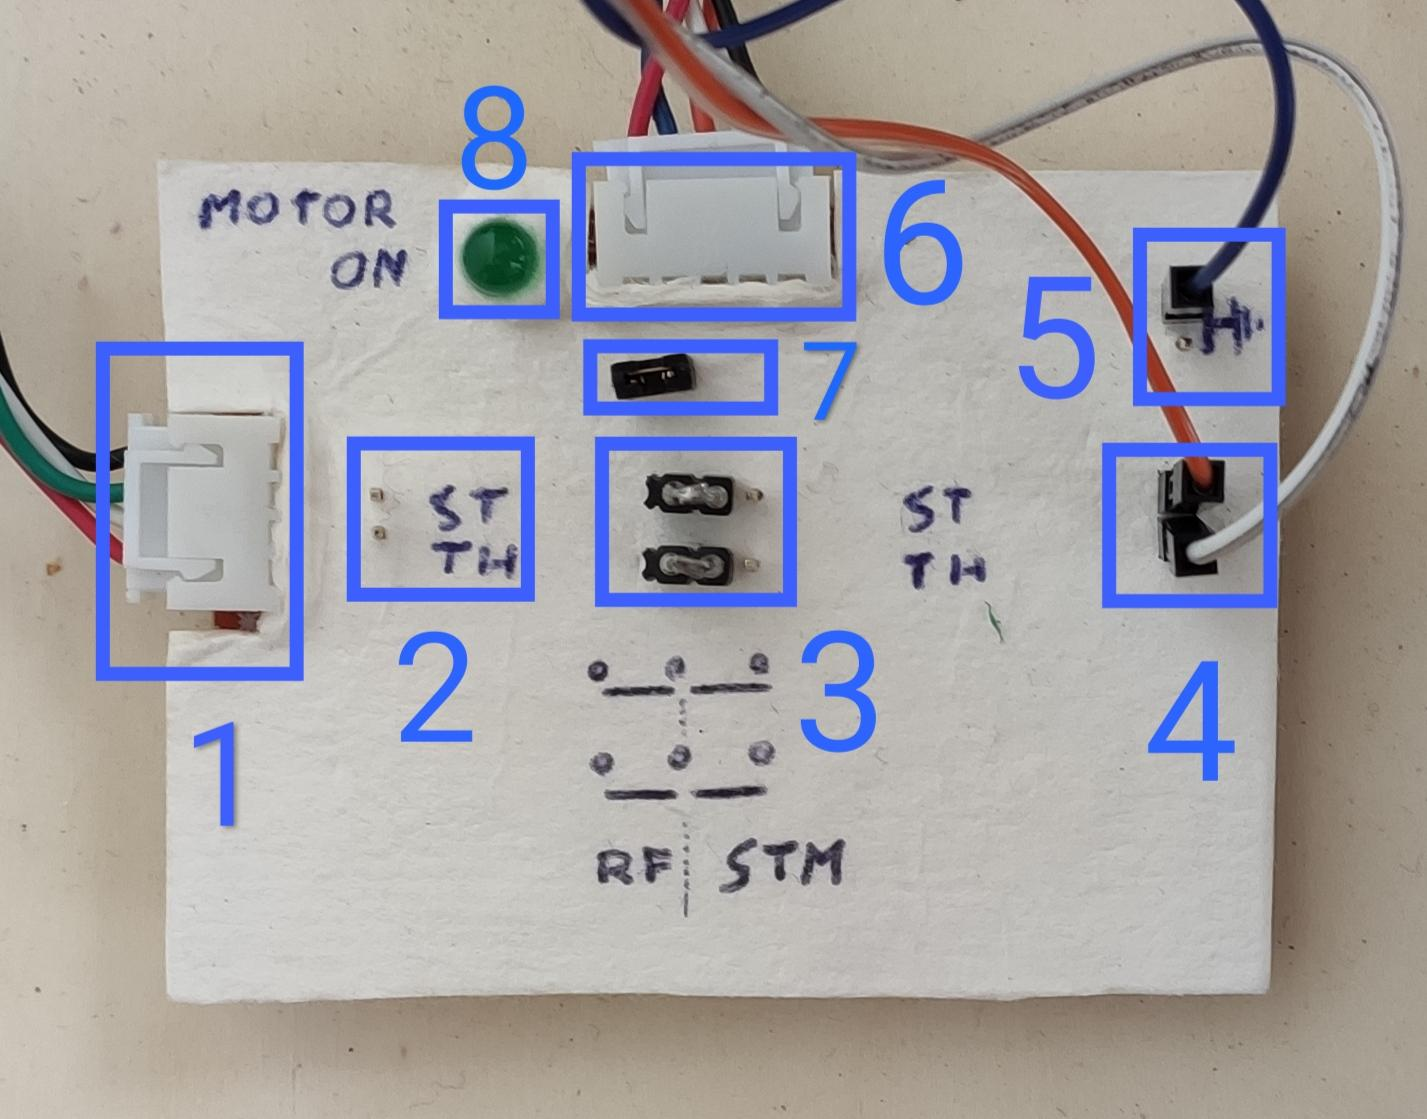
\includegraphics[width=0.45\textwidth]{pcb_controlli.png}
	\caption{PCB controlli}
	\label{fig:pcb_controlli}
\end{figure}


\begin{figure}
	\centering    
	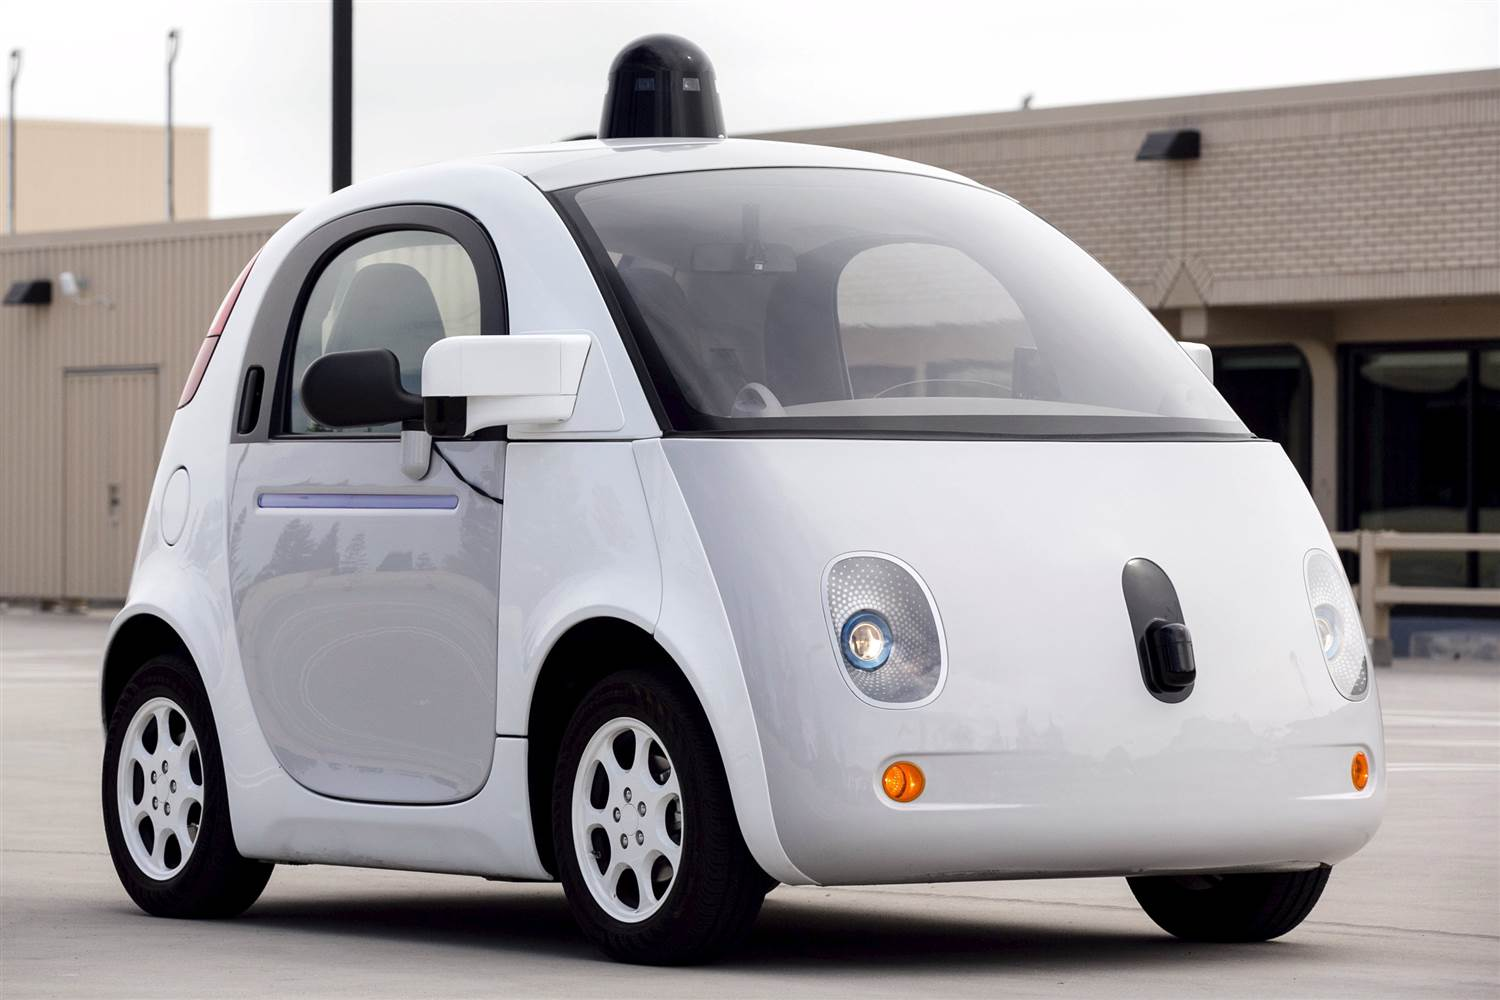
\includegraphics[height=0.2\textheight]{charlie_adulto.jpeg}
	\caption{Pinout del convertitore USB-seriale. \textbf{DA FARE!!!}}
	\label{fig: pinout usbserial}
\end{figure}


Il robot è dotato di due batterie:
\begin{itemize}
	\item LiPo \SI{14.8}{\volt} \SI{4200}{\milli \ampere \hour}, dedicata ad un’alimentazione generica, che viene sfruttata da tutti i componenti tranne i motori; da questa partono 3 linee di alimentazione: 
	\begin{itemize}
		\item a \SI{14.8}{\volt} per la STM
		\item a \SI{5}{\volt} per la Raspberry con connettore usb-c
		\item a \SI{5}{\volt} per fornire alimentazione ausiliaria all’HUB-USB
	\end{itemize}
	\item LiPo \SI{7.4}{\volt} \SI{6000}{\milli \ampere \hour} o NiMH \SI{7.2}{\volt} \SI{3000}{\milli \ampere \hour}, dedicate ai motori
\end{itemize}

I vari convertitori di tensione sono tutti installati su una PCB, posizionata all’interno di un box metallico.

Altro componente fondamentale \`e il convertitore usb-seriale ``TTL-232R-PCB'' prodotto da 
``Future Technology Devices International Ltd''. 
Questo consente di avere una linea di comunicazione seriale con la STM, attraverso la quale trasmettere informazioni necessarie all'algoritmo di navigazione.
Per conoscere quali informazioni vengono trasmesse, rifarsi alla sez.~\ref{sez:L'esperimento}, mentre per sapere la funzione dei vari pin, si consiglia di consultare il datasheet o, pi\`u comodamente, di rifarsi alla fig.~\ref{fig: pinout usbserial}. 
Per migliorare la semplicità di utilizzo ed evitare di incorrere in errori legati alle comunicazioni seriali, \`e stato associato al dispositivo ``TTL-232R-PCB'' il symlink \texttt{ttyUSBserial}, in modo tale che l’ordine di inizializzazione delle porte usb della raspberry non influenzi in alcun modo il nome del collegamento (per esempio: \texttt{ttyUSB0} oppure  \texttt{ttyUSB1})
Per conoscere i passaggi necessari alla realizzazione di tale symlink, si riporta la procedura dentro il file \texttt{/Info/renaming\_ttyUSB.txt}, fornito insieme al codice.


L'algoritmo implementato all'interno dell'STM non è l'unico mezzo attraverso il quale far muovere il veicolo: grazie alla presenza di una piccola PCB, sulla quale è presente il circuito adibito allo switch di sistema di controllo e al check dello stato dei motori, si ha la possibilità di utilizzare, alternativamente alla STM, un radiocomando per il controllo di sterzo e acceleratore.
Questa PCB, visibile in fig.~\ref{fig:pcb_controlli}, è dotata infatti di un led di stato verde che notifica quando l’alimentazione dei motori è attiva; sono inoltre presenti due jumper che permettono di scegliere tra STM e radiocomando come sorgente del controllo per sterzo e acceleratore. 
Sono sempre disponibili all’utente i contatti per potersi connettere e leggere quanto prodotto dal radiocomando.

\begin{enumerate}
    \item Connettore per il ricevitore del radiocomando;
    \item Pin per prelievo segnali PWM (steering/throttle) provenienti dal radiocomando;
    \item Jumper di selezione per la fonte di controllo: (jumper a sinistra) controllo da radiocomando e (jumper a destra) controllo da STM;
	\item Pin per connessione dei canali PWM provenienti da STM (steering/throttle);
    \item Pin per connessione GND comune;
    \item Connettore per i motori;
    \item Jumper di abilitazione alimentazione motori;
    \item LED di stato, indica quando l'alimentazione dei motori è attiva.
\end{enumerate}

Per ulteriori dettagli e approfondimenti sulle scelte che stanno dietro alle connessioni fatte, riferirsi a~\cite{ptvlocalizzazione}.
Lo schema completo è mostrato in fig.~\ref{fig:schema_completo}.

%--------------------------------------------------------
\subsection{Primo collegamento a Raspberry}
\label{sez: primo collegamento a raspberry}

Per iniziare a lavorare sulla raspberry in ssh, modalit\`a richiesta per gli esperimenti, \`e necessario impostare le connessioni WiFi a cui la raspberry si
connette automaticamente all'avvio. Per comodit\`a di utilizzo, suggeriamo di collegare la raspberry ad un monitor tramite un cavo microHDMI-HDMI e una tastiera/mouse usb.

Tutto il necessario da sapere riguardo i passaggi per il primo collegamento a raspberry si trovano nel file: \texttt{Info/README\_wifi\_settings.txt}, dei quali riportiamo qui un breve riassunto.
Come prima cosa è va impostato il WiFi: il file con le varie impostazioni WiFi, chiamato \texttt{interfaces}, si trova in \texttt{/etc/network/}. Per editarlo:
\begin{lstlisting}[style=bash]
	sudo nano /etc/network/interfaces
\end{lstlisting}
Questo file si occupa di leggere le configurazioni salvate nei file \texttt{.conf} di cui sono indicati i path al suo interno. 

Per aggiungere una nuova configurazione, inserire una riga per file \texttt{.conf} e commentare le altre (con \#).
Ad esempio, se volessimo aggiungere una configurazione di rete con nome "NOME\_RETE", \`e consigliato inserire la seguente riga all'interno del file (attenzione: l'ordine conta! Vengono tentate prima le connessioni alle reti riportate più in alto nel file):
\begin{lstlisting}[style=xml]
	wpa-conf /etc/wpa_supplicant/wpa_supplicant_NOME_RETE.conf
\end{lstlisting}
Il file \verb|wpa_supplicant_NOME_RETE.conf| deve contenere:
\begin{lstlisting}[style=xml]
	ctrl_interface=DIR=/var/run/wpa_supplicant GROUP=netdev
	update_config=1
	country=IT

	network={
		ssid="NOME_RETE"
		psk="password"
	}
\end{lstlisting}
e deve essere posizionato nel path specificato. 
Nel caso si usi quello di default, ovvero (\texttt{/etc/wpa\_supplicant/}), si riporta un comando utile per creare un nuovo file:
\begin{lstlisting}[style=bash]
	sudo nano /etc/wpa_supplicant/wpa_supplicant_NOME_RETE.conf
\end{lstlisting}

Al prossimo riavvio la raspberry si connetterà automaticamente alla prima rete configurata (in ordine di righe) che sia disponibile. 
Dato che è già in atto la connessione tramite lo schermo, che permette di visualizzare il contenuto di raspberry, suggeriamo come prima cosa di procedere con un backup della scheda originale: esiste un apposito tool all'interno di raspbian che consentirà di farlo agilmente. \`E buona norma creare il backup a monte dell'apporto di qualsiasi modifica o aggiunta, in quanto ciò consentirà di avere, in caso di necessità, un punto di ripristino funzionante. 

\subsection{Ros master/slave}
\label{sez: Ros master/slave}
Al fine di non sovraccaricare la raspberry e di avere un'interazione fluida con rviz e altri tool grafici di ros, è fortemente consigliato l'utilizzo di ros su altri computer in parallelo, delegando loro l'esecuzione dei task più costosi a livello computazionale (come appunto quelli grafici). 
Sono riportati di seguito i passaggi utilizzati da noi per impostare l'intero sistema, al fine di facilitare i nuovi utenti; per saperne di pi\`u consultare la \href{https://wiki.ros.org/ROS/Tutorials/MultipleMachines}{guida ufficiale}. 

Dopo svariate prove, siamo giunti alla conclusione che, per arrivare ad avere una interfaccia per utente sufficientemente fluida ed efficace, quello che dovevamo fare era avere il RosMaster su raspberry e utilizzare invece il pc per i tool grafici, esempio rviz o rqt. 
Per farlo, dobbiamo ottenere l'ip dei nostri dispositivi: è possibile farlo attraverso vari comandi (come \texttt{ifconfig} o \texttt{ip address}) e generalmente risulterà essere qulcosa del tipo: \verb|192.168.43.247|. 
Ipotizziamo quindi che l'ip della raspberry sia \texttt{IPrasp} e quello del pc \texttt{IPpc}. 
Adesso occorre modificare il file \texttt{.bashrc} sia su raspberry che su pc. Iniziamo da pc:
\begin{lstlisting}[style=bashpc]
	nano ~/.bashrc 
\end{lstlisting}
e inseriamo a fine file:
\begin{lstlisting}[style=xml]
	# ROS MASTER SU RASPBERRY, LATO PC
	export ROS_MASTER_URI=http://IPrasp:11311/
	export ROS_HOSTNAME=IPpc
	export ROS_IP=IPpc
\end{lstlisting}

Ripetiamo l'operazione su raspberry:
\begin{lstlisting}[style=bash]
	nano ~/.bashrc 
\end{lstlisting}
e quindi:
\begin{lstlisting}[style=xml]
	% # ROS MASTER SU RASPBERRY, LATO RASPBERRY
	% export ROS_MASTER_URI=http://localhost:11311/
	% export ROS_HOSTNAME=IPrasp
	% export ROS_IP=IPrasp
\end{lstlisting}

A questo punto, è sufficiente riavviare le shell dei terminali che si vogliono utilizzare: sarà possibile in essi lanciare i nodi, installati su pc, direttamente dal pc, ma sfruttando il master su raspberry.

%%%%%%%%%%%%%%%%%%%%%%%%%%%%%%%%%%%%%%%%%%%%%%%%%%%%%%%%%%%%%%%%%%%%%%%%%%%%%%%%%%%%%%%%%%%%%%%%%%%%%%
\section{RPlidar}
\begin{figure}[] 
	\centering    
	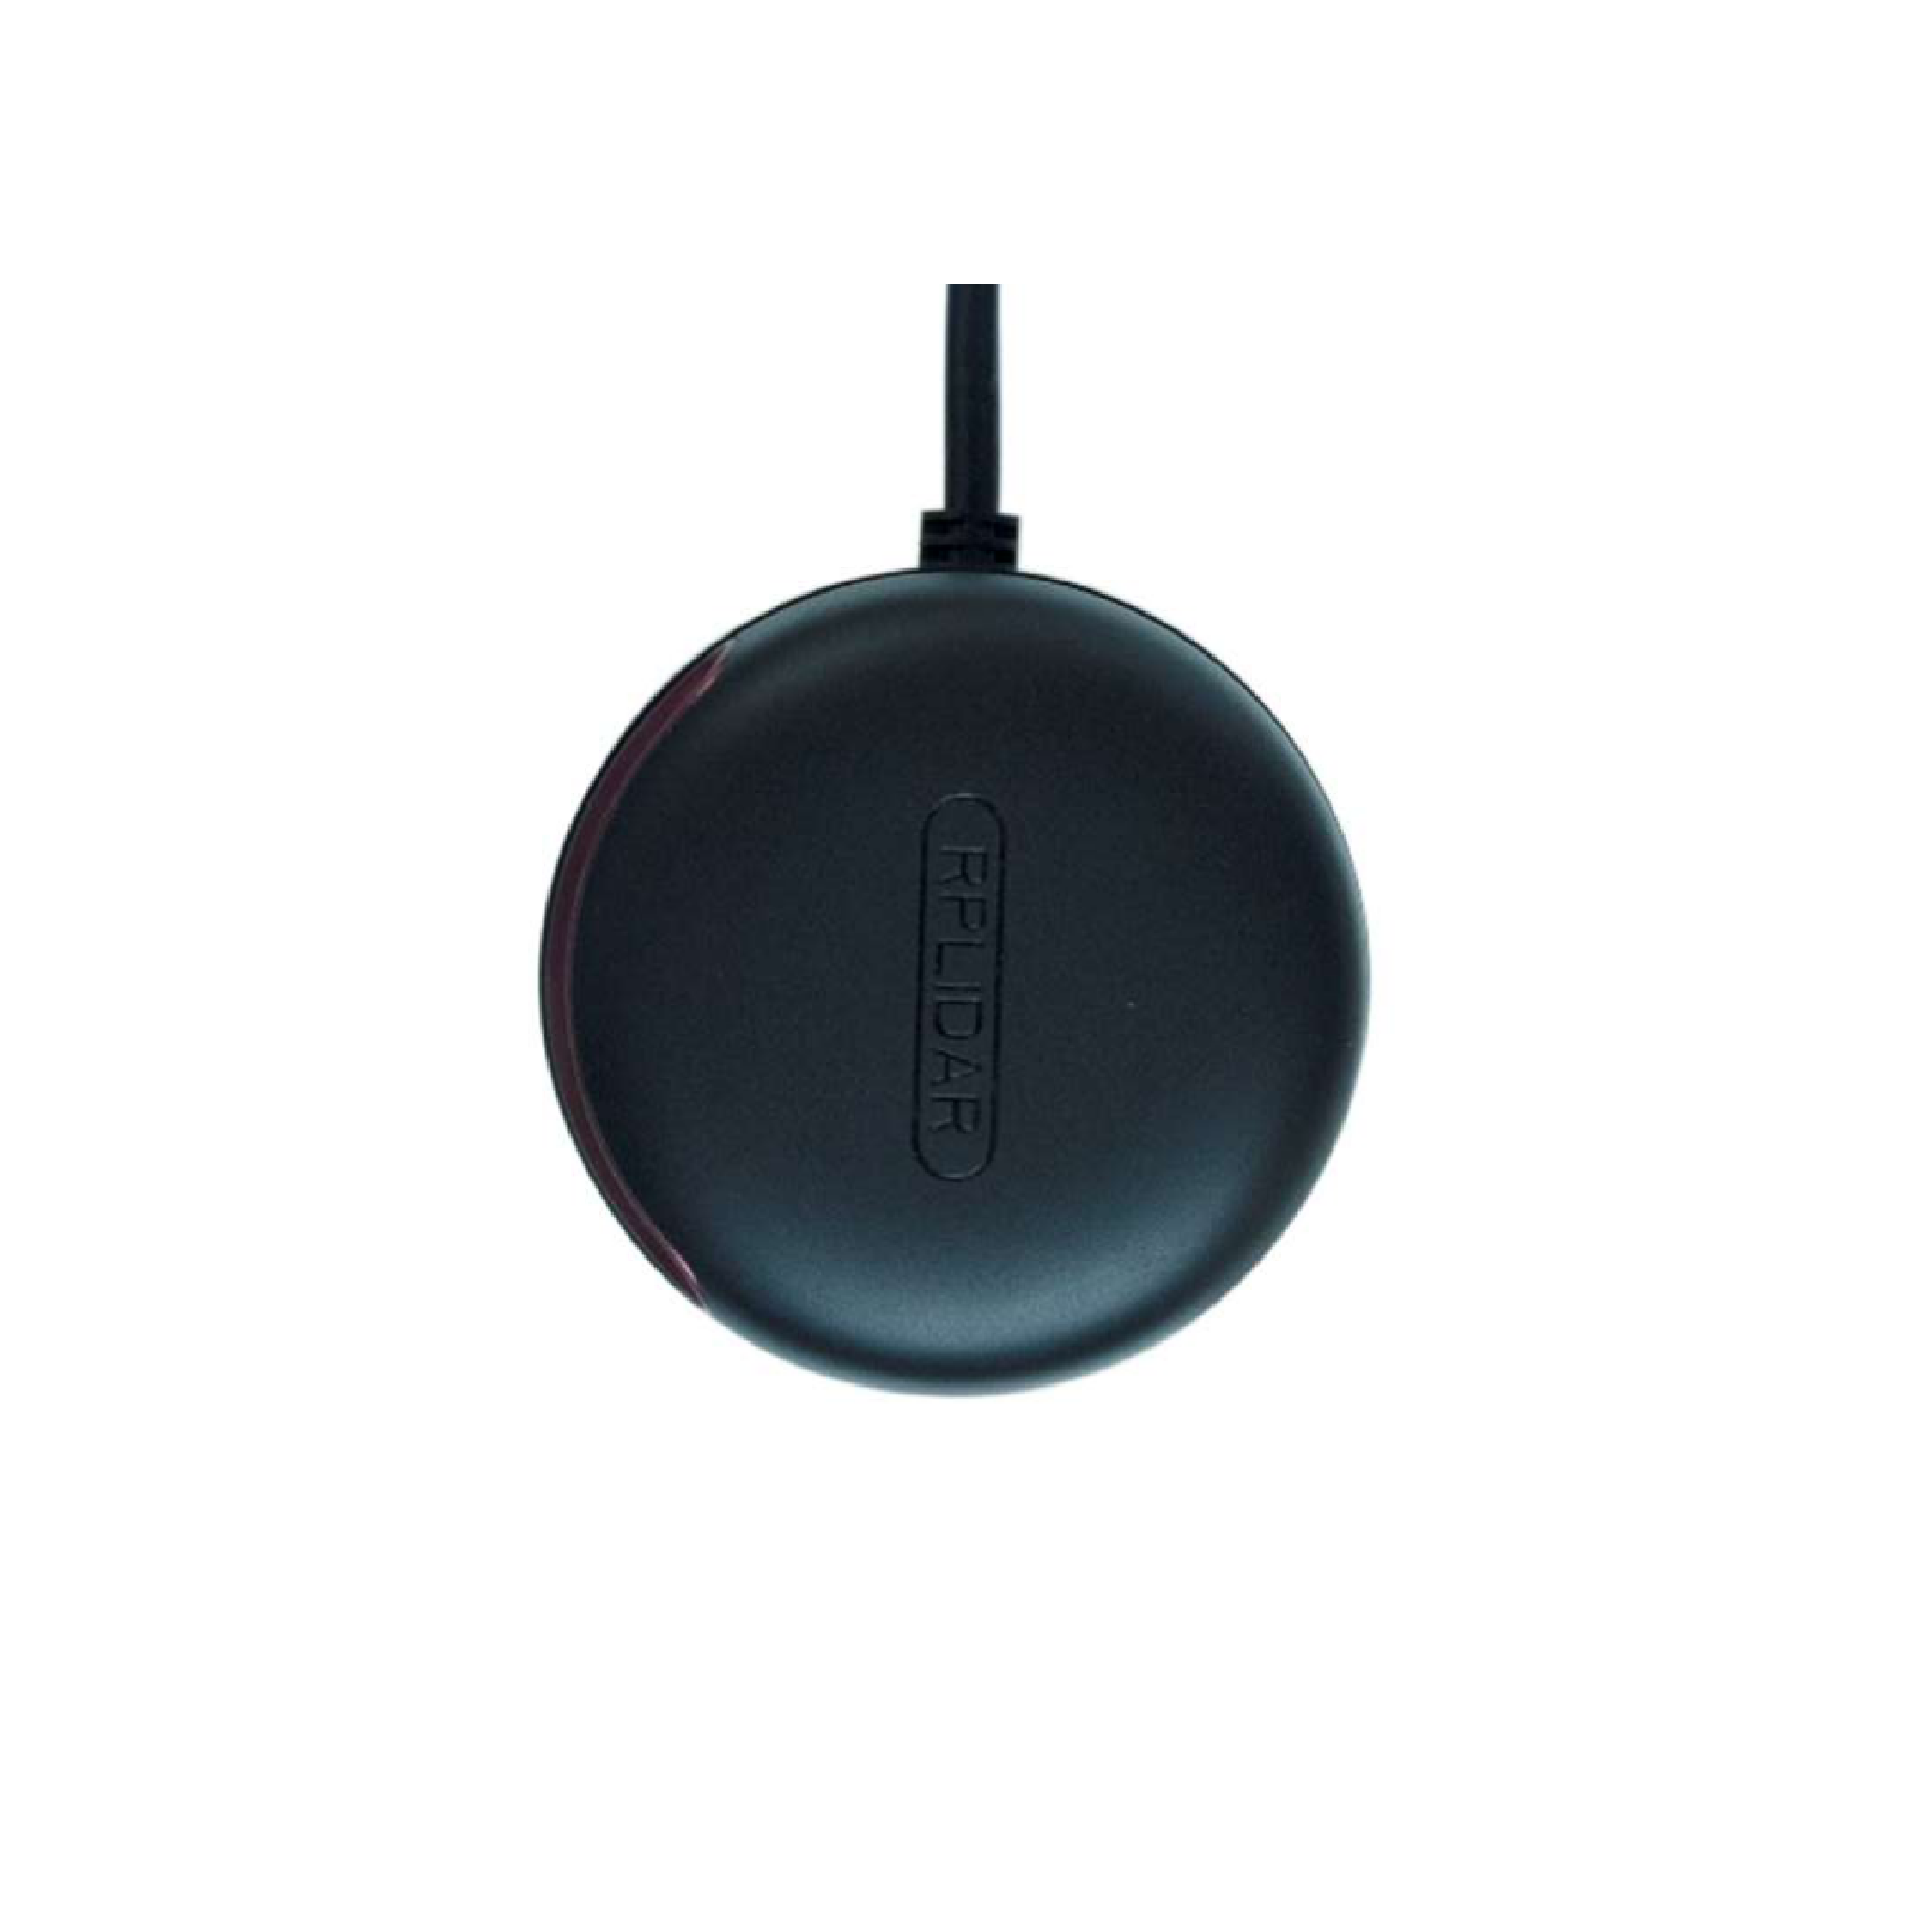
\includegraphics[height=.2\textheight]{rplidar_axis.pdf}
	\caption{Riferimenti  \textbf{DA EDITARE}}
	\label{fig: rplidar axis}
\end{figure}

Il lidar utilizzato su Charlie \`e un RPlidar A3 prodotto da Slamtec, documentazione e caratteristiche sono disponibili sulla \href{https://www.slamtec.com/en/Lidar/A3}{pagina} del produttore.
Per quanto riguarda il codice, abbiamo scelto di utilizzare il \href{https://wiki.ros.org/rplidar}{pacchetto} ros sviluppato proprio da Slamtec. 
Alcune accortezze hardware sono state:

\begin{itemize}
	\item utilizzare un cavo micro usb di buona qualit\`a. Infatti questo cavo \`e responsabile sia dell'alimentazione del motore brushless sia della seriale di comunicazione.
			Ci siamo accorti che se il voltaggio in ingresso al lidar cala sotto i \SI{4.7}{\volt} la comunicazione seriale si interrompe e non \`e pi\`u possibile sfruttare i nodi ros
			di RPlidar.

	\item orientare correttamente il sistema di riferimento del lidar, in quanto le rappresentazioni nel datasheet sono invertite di $\pi$. 
	L'asse x ($\vartheta = 0$) infatti coincide con l'uscita del cavo dalla struttura principale come si pu\`o vedere in fig.~\ref{fig: rplidar axis}.

	\item cercare di far vibrare il meno possibile la struttura di sostegno e rialzo del lidar.

\end{itemize}

Per evitare che l'ordine di inizializzazione delle porte usb della raspberry non influenzasse il nome del collegamento (per esempio: \texttt{ttyUSB0} oppure \texttt{ttyUSB1})
abbiamo realizzato il symlink \texttt{ttyUSBlidar} in modo tale che la porta seriale del lidar sia sempre chiamata \texttt{ttyUSBlidar}. 
Su come si realizzi tale symlink abbiamo riportato la procedura dentro il file \texttt{/Info/renaming\_ttyUSB.txt}.

In ambiente ros viene eseguito il lidar andando a lanciare il nodo \texttt{rplidarNode} che pubblica sul topic \texttt{/scan}. 
\`E stato sviluppato il file di lancio \texttt{rplidar\_a3.launch} con i parametri opportuni.  
Per quanto riguarda l'utilizzo del lidar non \`e stato necessario alcun sviluppo software in quanto il pacchetto ros risulta gi\`a completo.


%%%%%%%%%%%%%%%%%%%%%%%%%%%%%%%%%%%%%%%%%%%%%%%%%%%%%%%%%%%%%%%%%%%%%%%%%%%%%%%%%%%%%%%%%%%%%%%%%%%%%%
\newpage
\section{Sistema Pozyx}
\label{sez:Sistema Pozyx}

\begin{figure}[h]
	\centering
	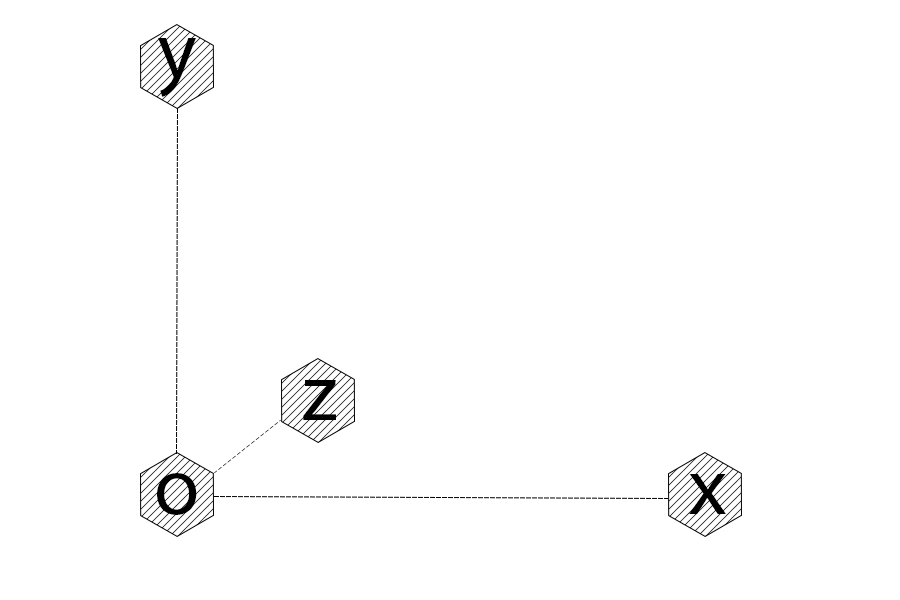
\includegraphics[height=0.2\textheight]{uwb_axis.png}
	\caption{Disposizione ancore}
	\label{fig: disposizione ancore}
\end{figure}


Il Pozyx è un sistema di localizzazione alternativo al GPS, basato sulla tecnologia ultra-wideband
(UWB). In breve, si tratta di una tecnica di trasmissione sviluppata per la trasmissione e la ricezione di segnali 
sfruttando degli impulsi di energia a radiofrequenza di durata temporale molto ridotta (nanosecondi) con conseguente
banda spettrale ampia.
Nel sistema Pozyx si possono distinguere due entità: le ancore e le tag.
La configurazione base prevede l'utilizzo 4 ancore, che fungono da dispositivi fissi, e un tag, che rappresenta il dispositivo mobile.
Grazie all'utilizzo di un algoritmo di triangolazione, il tag si può localizzare rispetto alle ancore. Teoricamente, la localizzazione 
effettuata sfruttando la tecnologia ultra-wideband permette di ottenere un posizionamento con una accuratezza al centimetro anche
in ambienti indoor e in presenza di ostacoli di natura non metallica, condizioni sfavorevoli per la natura fisica del sistema (che presenta 
migliori performance in ambienti aperti ed ampi, privi di oggetti metallici e ostacoli sui quali possano verificarsi fenomeni di scatterning 
del segnale inviato). 
Sia all'interno delle tag che delle ancore è presente un microcontrollore, nel quale vengono eseguiti la maggior parte dei task richiesti,
come gli algoritmi di triangolazione e autocalibrazione. A lui è demandata anche la gestione dell’interfaccia con dispositivi esterni
(come Arduino).
Solo nel caso delle tag, che per questo sono utilizzate come dispositivi mobili, sono presenti i seguenti sensori: un magnetometro, un giroscopio, un
accelerometro e un sensore di pressione (altimetro). I dati dei sensori vengono utilizzati dal microcontrollore
per la triangolazione e sono disponibili all’utente.
Per quanto riguarda l'utilizzo di tale sistema di posizionamento, è necessario prima di tutto predisporre l'ambiente di lavoro.
La prima cosa da fare è posizionare le ancore in modo tale che delimitino uno spazio entro il quale il sistema di localizzazione
funzioni correttamente. Il miglior modo di disporle è quello di metterle in alto e sulla line-of-sight dell’utente: questo tipo di scelta
aumenta infatti la possibilità di ricevere un buon segnale in quanto si limita la presenza di possibili ostacoli. 
Per un buon funzionamento e per ridurre il più possibile l'errore di posizionamento, è consigliato inoltre distribuire le ancore affinché tutte le 
direzioni siano coperte.
Nel caso, infatti, in cui gli ancoraggi si trovino su una linea retta, l'errore di posizionamento risultante sarà molto grande e potranno
verificarsi ambiguità di posizione legate alla simmetria della configurazione.
Importante sottolineare che le ancore devono essere disposte verticalmente con l’antenna UWB rivolta verso l’alto.

Per tutte le operazioni che vengono richieste tra le ancore e le tag, è necessario specificare tra quali dispositivi lavorare. 
Con l'identificativo assegnato al campo \verb|remote_id|, si dichiara la tag o l'ancora sulla quale vogliamo usare le funzioni di registro. Nel caso (di default)
in cui questo sia settato al valore \verb|None|, verrà usata la tag locale, ovvero quella connessa al pc (su cui viene utilizzata la seriale).
Presa ad esempio la funzione doRanging(destination, \verb|device_range|, \verb|remote_id=None|), essa effettua una misurazione della distanza tra i dispositivi i cui identificativi sono
\verb|remote_id| e destination. Lasciando il valore di default per \verb|remote_id|, cioè \verb|None|, la distanza viene automaticamente valutata tra il dispositivo connesso alla seriale del PC e il
dispositivo il cui identificativo è destination. 
Se si desidera invece che il ranging venga effettuato tra due diversi dispositivi della rete basterà inserire l’opportuno valore di \verb|remote_id|.

Nel nostro caso, questo aspetto è importante nel momento in cui vengono prelevate le posizioni relative delle ancore nella configurazione attuale. Con \verb|remote_id=None| chiediamo di fatto
alla tag connessa in seriale ad Arduino le informazioni delle ancore, ovvero leggiamo sul suo chip i valori relativi all'ancora richiesta (posizione, id...).
Per questo motivo, ad ogni nuovo avvio del sistema è necessario salvare all'interno delle tag i valori di posizione più recenti delle ancore, ovvero gli ultimi salvati all'interno delle ancore stesse
al termine del processo di autocalibrazione.
Affinché il sistema funzioni è infatti necessario che ogni ancora abbia coscienza della sua posizione rispetto alle altre ancore: la procedura di autocalibrazione è quella utilizzata a tale scopo.
Per informazioni inerenti alla procedura adottata, vedere app.~\ref{sez:Autocalibrazione}. Per come funziona l'algoritmo, l'ancora 0 è quella scelta come origine del frame UWB che verrà costruito. 
L'ancora 1 è quella che fornisce la direzione dell'asse y, ovvero le cui coordinate finali saranno \begin{verbatim}(0, y1, 0)\end{verbatim}, mentre l'ancora 2 quella dell'asse x. La quarta ancora, 
posizionata a una altezza diversa dalle altre 3 (che devono invece essece complanari), evidenzia la direzione dell'asse z.




infine, è importante verificare che siano assenti eventuali interferenze elettromagnetiche tra i dispositivi, le quali, specialmente se interposte tra le ancore, 
possono rendere difficile la comunicazione tra i dispositivi della rete.
********

* tag
* anchors, come disporre le ancore \\
* autocalibrazione
* come gestire flash memory dei device
* warning: remote\_id 
		problematiche relative al doPositioning veloce (servono le pause)
		pacchetto ros custom descrivere in breve cosa fanno i file dentro charlie\_pozyx

%%%%%%%%%%%%%%%%%%%%%%%%%%%%%%%%%%%%%%%%%%%%%%%%%%%%%%%%%%%%%%%%%%%%%%%%%%%%%%%%%%%%%%%%%%%%%%%%%%%%%%
\section{Sistema Vicon}
\label{sez:Sistema Vicon}

Il sistema Vicon \`e un sistema molto accurato di motion capture. 
In questo progetto \`e stato usato per fornire un \textit{ground-truth} e un confrotno all'algoritmo di navigazione. 
In tal senso quindi abbiamo ritenuto opportuno sviluppare i nodi e i topic di dialogo con il sistema Vicon all'esterno del workspace della raspberry: infatti questi si trovano su pc nel pacchetto in \texttt{charlie\_remote}.

Per poter dialogare con il sistema Vicon \`e sufficiente includere nel proprio \texttt{catkin\_ws} il pacchetto \texttt{vrpn\_client\_ros} disponibile sulla \href{https://wiki.ros.org/vrpn_client_ros}{wiki.ros} e scaricabile dalla \href{https://github.com/ros-drivers/vrpn_client_ros}{repo GitHub}.
Questo pubblicher\`a la posa, il twist e l'accelerazione di ogni oggetto selezionato nel software di tracking (maggiori dettagli su quali oggetti selezionare nelle sezioni \ref{sez:L'esperimento} e \ref{sez: Guida breve all'esperimento}).

\subsubsection*{Creazione oggetto}
Nonostante ci siano gi\`a gli oggetti necessari per il tracking di Charlie riportiamo la procedura di creazione di un nuovo oggetto che pu\`o essere utile in caso di modifiche ai marker o in altre circostanze. 
Sinteticamente:
\begin{enumerate}
	\item Disporre 4 o pi\`u marker sull'oggetto desiderato in modo asimmetrico. Per facilitare i prossimi passi disporre alcuni marker sugli assi del sistema di riferimento body.
	
	\item Selezionare i marker nell'applicazione ``Vicon Tracker 3.7.0 x64'' semplicemente clickando e tenendo premuto il tasto sinistro del mouse, poi premere pausa (pulsante collocato a sinistra).
	
	\item spostarsi nel tab Objects, assegnare un nome in basso e premere Create Object. L'applicazione assegna un sistema locale di default.
	
	\item Modificare il sistema locale premendo sugli assi o andando nelle propriet\`a dell'oggetto appena creato. Una volta soddisfatti premere \texttt{Ctrl+S} per salvare l'oggetto.
	
	\item Premere di nuovo il pulsante di pausa e verificare che il tracciamento stia funzionando.
\end{enumerate}

\subsubsection*{Calibrazione}
Per effettuare una calibrazione del sistema, necessaria di tanto in tanto \`e necessario utilizzare la wand. 
Per prima cosa accedere all'applicazione ``Vicon Tracker 3.7.0 x64'' e collocarsi nella tab ``Calibrate''. 
Premere su ``Start'' nella sezione ``CALIBRATE CAMERAS'', avviando cos\`i la procedura di autocalibrazione: spostare la wand con pattern circolari all'interno della stanza assicurandosi di avere sempre pi\`u camere ``a vista''. 
Il software interromper\`a da solo l'acquisizione dei dati una volta che questi siano sufficienti.

Adesso \`e necessario definire il sistema di riferimento. Per far questo andiamo a posizionare l'incrocio degli assi della wand nel punto in cui vogliamo l'origine e gli assi stessi allineati con gli assi-Vicon desiderati.
Selezioniamo quindi il marker all'incrocio come origine e gli altri marker come asse x e asse y completando cos\`i la calibrazione del sistema. 
Nella stanza volo il sistema di riferimento pi\`u usato \`e rappresentato in fig.REF.
\textbf{FARE IMMAGINEEE}


%%%%%%%%%%%%%%%%%%%%%%%%%%%%%%%%%%%%%%%%%%%%%%%%%%%%%%%%%%%%%%%%%%%%%%%%%%%%%%%%%%%%%%%%%%%%%%%%%%%%%%
\newpage
\section{L'esperimento}
\label{sez:L'esperimento}
procedura con i comandi, ogni cosa che facciamo \`e commentata e descritta \\
topic \texttt{/scan} letto da hector\_slam produce mappa e da scan\_tools produce la tf da laser odom a base\_link \\
albero nodi\\
albero tf\\

\subsection{Sistema di riferimento body}
\textbf{FARE FIGURINAAAAAAAAAAAAAAAAA}

%%%%%%%%%%%%%%%%%%%%%%%%%%%%%%%%%%%%%%%%%%%%%%%%%%%%%%%%%%%%%%%%%%%%%%%%%%%%%%%%%%%%%%%%%%%%%%%%%%%%%%
\section{Prove?}
\subsection{Confronto Vicon}

\subsection{Esperimento nel cortile}

\subsection{Esperimento all'aperto}



%%%%%%%%%%%%%%%%%%%%%%%%%%%%%%%%%%%%%%%%%%%%%%%%%%%%%%%%%%%%%%%%%%%%%%%%%%%%%%%%%%%%%%%%%%%%%%%%%%%%%%
\newpage
\section{Guida breve all'esperimento}
\label{sez: Guida breve all'esperimento}
In questa sezione \`e scritta, in modo molto sintetico, la procedura per lanciare un esperimento. Per una guida dettagliata rifarsi a sez.~\ref{sez:L'esperimento}. 

Prima di tutto \`e necessario disporre le ancore come descritto in sez.~\ref{sez:Sistema Pozyx} e come si pu\`o vedere in fig.~\ref{fig: disposizione ancore}. Assicurarsi di aver impostato correttamente le impostazioni WiFi (sez.~\ref{sez: primo collegamento a raspberry}) e di avere il PC e la Raspberry connessi alla stessa rete WiFi.


Connettersi \textbf{ssh} alla Raspberry dal PC digitando da terminale del PC, con password \texttt{robot}:
\begin{lstlisting}[style=bashPC]
	ssh -X -C pi@raspberrypi.local		# avvia ssh
\end{lstlisting}

Per l'\textbf{autocalibrazione} (necessaria ogni volta che viene riposizionato il sistema di ancore) lanciare 
dalla cartella \texttt{home} (da terminale della Raspberry):
\begin{lstlisting}[style=bash]
	python3 ~/charlie_autocalibration/autocalibration_ransac.py
\end{lstlisting}
infine rispondere ``y'' per salvare i risultati nella memoria flash delle ancore.

Adesso \`e necessario avviare il \textbf{posizionamento} delle tag pozyx e la comunicazione \textbf{seriale} con Icaro (suggeriamo di utilizzare pi\`u terminali con \href{https://terminator-gtk3.readthedocs.io/en/latest/}{terminator}):
\begin{lstlisting}[style=bash]
	roslaunch charlie_launch start_uwb.launch		# avvia uwb
	roslaunch charlie_launch start_serial.launch	# avvia seriale con stm
\end{lstlisting}

\subsection*{Nuova Mappa}
Una nuova mappa \`e necessaria quando si cambia posizionamento alle ancore o banalmente si cambia luogo. Consigliamo di muovere Charlie attraverso il radiocomando in questa fase.
\begin{lstlisting}[style=bash]
	roslaunch charlie_launch save_map_origin.launch		# con Charlie fermo!
	roslaunch charlie_launch new_map.launch 	# muovere Charlie lentamente
\end{lstlisting}

Una volta soddisfatti del risultato salvare la mappa attraverso:
\begin{lstlisting}[style=bash]
	cd charlie_ws/maps
	rosrun map_server map_saver -f NOME_MAPPA
\end{lstlisting}

\subsection*{Localizzazione}
Sostituire il nome della mappa che si vuole utilizzare nel file

\verb|/home/pi/charlie_ws/src/charlie_launch/launch/localization.launch|:

\begin{lstlisting}[style=xml, firstnumber=14]
	<arg name="file_NUM" default="NOME_MAPPA" />
	<node name="map_server" pkg="map_server" type="map_server" args="$(arg path)$(arg file_NUM).yaml"/>
\end{lstlisting}

Quindi lanciare:
\begin{lstlisting}[style=bash]
	roslaunch charlie_launch localization.launch
\end{lstlisting}

Nello stesso file \`e possibile impostare di visualizzare rviz attraverso la connessione ssh con il ``Compressed X11 Forwarding '' scommentando la riga corrispondente di rviz. Questa opzione \`e molto sconsigliata da noi in quanto rende la visione poco reattiva. Per ovviare a questo problema, dopo aver configurato pc e raspberry come descritto in sez.~\ref{sez: Ros master/slave}, \`e possibile lanciare da pc:

\begin{lstlisting}[style=bashPC]
	roslaunch charlie_remote rviz_remote.launch
\end{lstlisting}
In questo momento l'esperimento \`e iniziato!

\subsection*{Waypoints}
\`E possibile indicare una posa-goal tramite il comando \texttt{2DNavgoal} direttamente da rviz (tenere premuto per assegnare l'orientazione).
Per attivare i motori e permettere al robot di spostarsi, pubblicare il seguente messaggio sul topic \verb|start\_and\_stop|:

\begin{lstlisting}[style=bash]
	rostopic pub /start_and_stop std_msgs/Float64 "data: 1.0"
\end{lstlisting}

e per fermarli:

\begin{lstlisting}[style=bash]
	rostopic pub /start_and_stop std_msgs/Float64 "data: 0.0"
\end{lstlisting}

\subsection*{Sistema Vicon}
Ovviamente per utilizzare il sistema Vicon \`e necessario essere nella stanza del volo. 
Per l'installazione rifarsi a sez.~\ref{sez:Sistema Vicon}. 
Una volta che il sistema \`e in funzione, avviare l'applicazione ``Vicon Tracker 3.7.0 x64'' e selezionare nella lista oggetti: \texttt{Charlie} e \texttt{Active Wand v2 (Origin Tracking)}. 
Connettere il computer fisso connesso fisicamente al sistema Vicon (che sar\`a il server Vicon) alla stessa rete di raspberry e pc e in seguito modificare nel file di lancio \texttt{charlie\_remote/launch/vicon\_charlie.launch} l'ip del server Vicon nella seguente riga:
\begin{lstlisting}[style=xml, firstnumber=6]
	<arg name="server" default="IP_SERVER"/>
\end{lstlisting}

Per avviare i dialoghi tra ros e il sistema Vicon avviare da pc:
\begin{lstlisting}[style=bashPC]
	roslaunch charlie_remote vicon_charlie.launch
\end{lstlisting}

poi salvare la trasformazione tra vicon e uwb (all'utente \`e richiesto di posizionare la wand in successione sulle ancore):
\begin{lstlisting}[style=bashPC]
	rosrun charlie_remote vicon2uwb_tf.py
\end{lstlisting}

e infine lanciare il nodo che pubblica la posizione di Charlie in frame map:
\begin{lstlisting}[style=bashPC]
	rosrun charlie_remote charlie_vicon2map.py
\end{lstlisting}


\subsection*{Rosbag}
Per registrare i dati attraverso una rosbag suggeriamo di non sottoscriversi a tutti i topic ma di lanciare il seguente comando da pc (dopo essersi spostati nella cartella desiderata):
\begin{lstlisting}[style=bashPC]
	rosbag record /clock /initialpose /map /orientation /particlecloud /robot_pose /rosout /rosout_agg /scan /tag_center /tf /amcl_pose /charlie_vicon_map -O NOME_BAG.bag
\end{lstlisting}

Per eseguire i topic necessari a AMCL, prima riconfigurare il file:

\verb|../charlie_remote/launch/exec_bag.launch| con i file e il path che si vogliono utilizzare e quindi lanciare da pc:
\begin{lstlisting}[style=bashPC]
	roslaunch charlie_remote exec_bag.launch
\end{lstlisting}
e da raspberry (modificando il nome della mappa da utilizzare all'interno del file di lancio \verb|localization_bag.launch|):
\begin{lstlisting}[style=bash]
	roslaunch charlie_launch localization_bag.launch
\end{lstlisting}

%%%%%%%%%%%%%%%%%%%%%%%%%%%%%%%%%%%%%%%%%%%%%%%%%%%%%%%%%%%%%%%%%%%%%%%%%%
\newpage
\appendix
\section{Autocalibrazione ancore Pozyx}
\label{sez:Autocalibrazione}
L'autocalibrazione si basa sullo script \texttt{python3} ``autocalibration\_ransac.py''. 
Per farlo funzionare occorre per prima cosa avere quattro ancore correttamente alimentate ed un dispositivo Pozyx connesso, il quale servirà da comunicazione seriale tra la rete Pozyx e l’utente. 
Il dispositivo seriale può, a discrezione dell’utente, essere un’ancora o un tag. 
É possibile, se si desidera, effettuare una calibrazione manuale delle ancore, andando a settare la variabile \verb|autoCal| a \verb|True|. 
In tal caso si dovrà utilizzare un metro per misurare la distanza relativa tra le coppie di ancore della rete ed inserire manualmente i valori misurati nelle opportune variabili \texttt{r01}, \texttt{r02}, \texttt{r03}, \texttt{r12}, \texttt{r13} ed \texttt{r23}, che rappresentano le distanze tra le rispettive antenne.
Per quanto riguarda invece la calibrazione automatica, lo script prevede una fase di acquisizione dei dati necessari, successivamente viene eseguito l’algoritmo ransac ed infine viene utilizzato l’algoritmo algebrico per determinare le coordinate effettive delle ancore. 
L’algoritmo ransac rimuove eventuali outliers dalle misurazioni delle distanze relative tra le antenne e fornisce quindi una stima della distanza tra ciascuna coppia di ancore basata sui dati senza outliers.
Nel corso della procedura di autocalibrazione vengono stampati sul terminale vari dati, tra cui i fondamentali sono:
\begin{itemize}
	\item Coordinate dei dispositivi all’accensione del sistema, prima che sia effettuata la nuova calibrazione;
	
	\item Risultato del settaggio dei parametri UWB della rete;
	
	\item Il risultato dell’algoritmo ransac per la distanza tra le ancore;
	
	\item Risultato dell'algoritmo algebrico per determinare le coordinate delle ancore: in caso di fallimento dell'algoritmo, \`e mostrato su terminale l'errore;
\end{itemize}

Una volta terminata la calibrazione, sia questa stata manuale o automatica, ciascuna ancora avrà
salvato nella propria lista dei dispositivi le proprie coordinate, ossia conoscerà le proprie coordinate. 
Questi dati sono salvati permanentemente nella memoria flash.
In una successiva fase di positioning è quindi buona norma che il dispositivo che si deve localiz-
zare interroghi le ancore per conoscere la loro posizione e crei quindi una propria lista interna dei
dispositivi della rete.


Per maggiori dettagli, fare riferimento al dettagliato lavoro~\cite{ctesconistudio}.

% Bibliography
\newpage
\bibliography{biblio}


\end{document}